\section{Implementation of a QECC}
\label{sec:implementation}

In this section we are finally using the tools and methods presented in the last section to apply the quantum error correction (bit-flips) for the quantum Fourier transform.

\subsection{Implementing the quantum Fourier transform circuit}
\label{subsec:implementing-quantum-fourier-transform-circuit}

First and foremost it would make certainly sense to build the proposed QFT circuit and see if it actually works on a simulator and a real quantum device.
Recalling the basic concepts chapter we have already seen a generic circuit in figure~\ref{fig:qft-generic-circuit} that can be rebuilt using Qiskit.
The controlled \texttt{R}-gate is a rotation around the Z-axis which can be realized in \texttt{Qiskit} using a controlled \texttt{U1} gate~\cite{ControlledU1Gate}.

Before using \emph{Qiskit} and building the circuit we need to set up the code by listing the needed imports in appendix~\ref{subsec:qft-circuit-qiskit-necessary-imports} for \emph{Python}.
Afterwards we can follow the circuit in figure~\ref{fig:qft-generic-circuit} and implement it iteratively for any size in Qiskit as seen in appendix~\ref{subsec:qft-function}.
That allows us creating an arbitrarily big circuit.
One example circuit graph for 4 input qubits is created and shown in figure~\ref{fig:qft-4-qubit-circuit}.
Note that the circuit is mirrored vertically compared to the reference circuit, as Qiskit is ordering the qubits differently compared to most resources~\cite{QiskitGettingStarted}.

\begin{figure}[H]
    \centering
    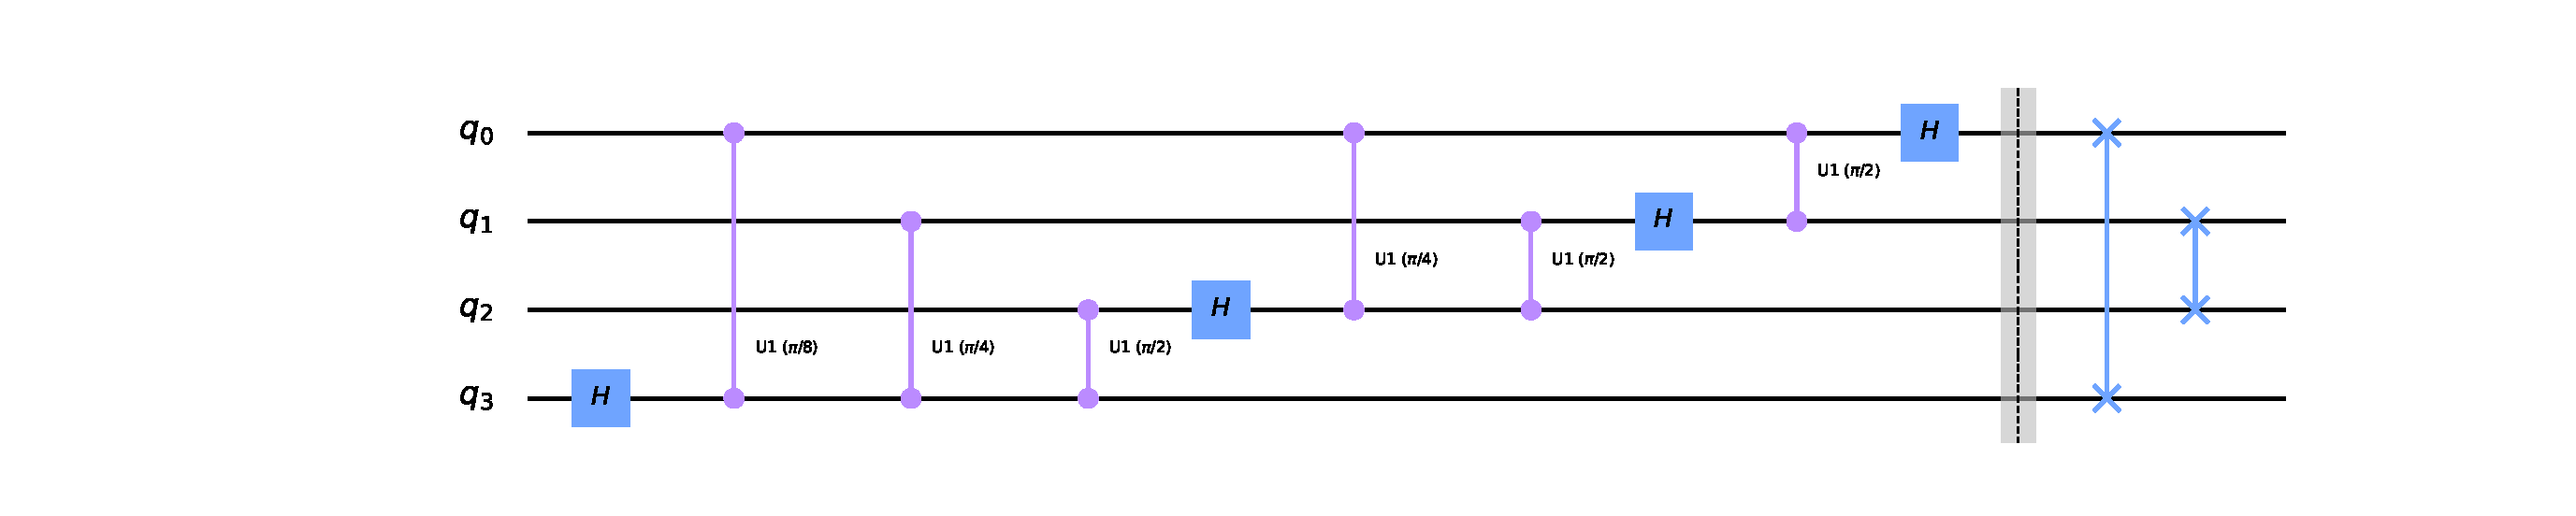
\includegraphics[width=\textwidth]{res/qft-4-qubits-circuit.pdf}
    \caption{Qiskit 4-qubit QFT circuit graph}
    \label{fig:qft-4-qubit-circuit}
\end{figure}

To get the inverse of that circuit \emph{Qiskit} offers the method \texttt{inverse()} which can be applied on any \texttt{QuantumCircuit}.
It is applied in the function displayed in appendix~\ref{subsec:inverse-qft-function} and delivers together with the non-inversed QFT the circuit depicted in figure~\ref{fig:qft-4-qubit-circuit-with-inverse}.

\begin{figure}[H]
    \centering
    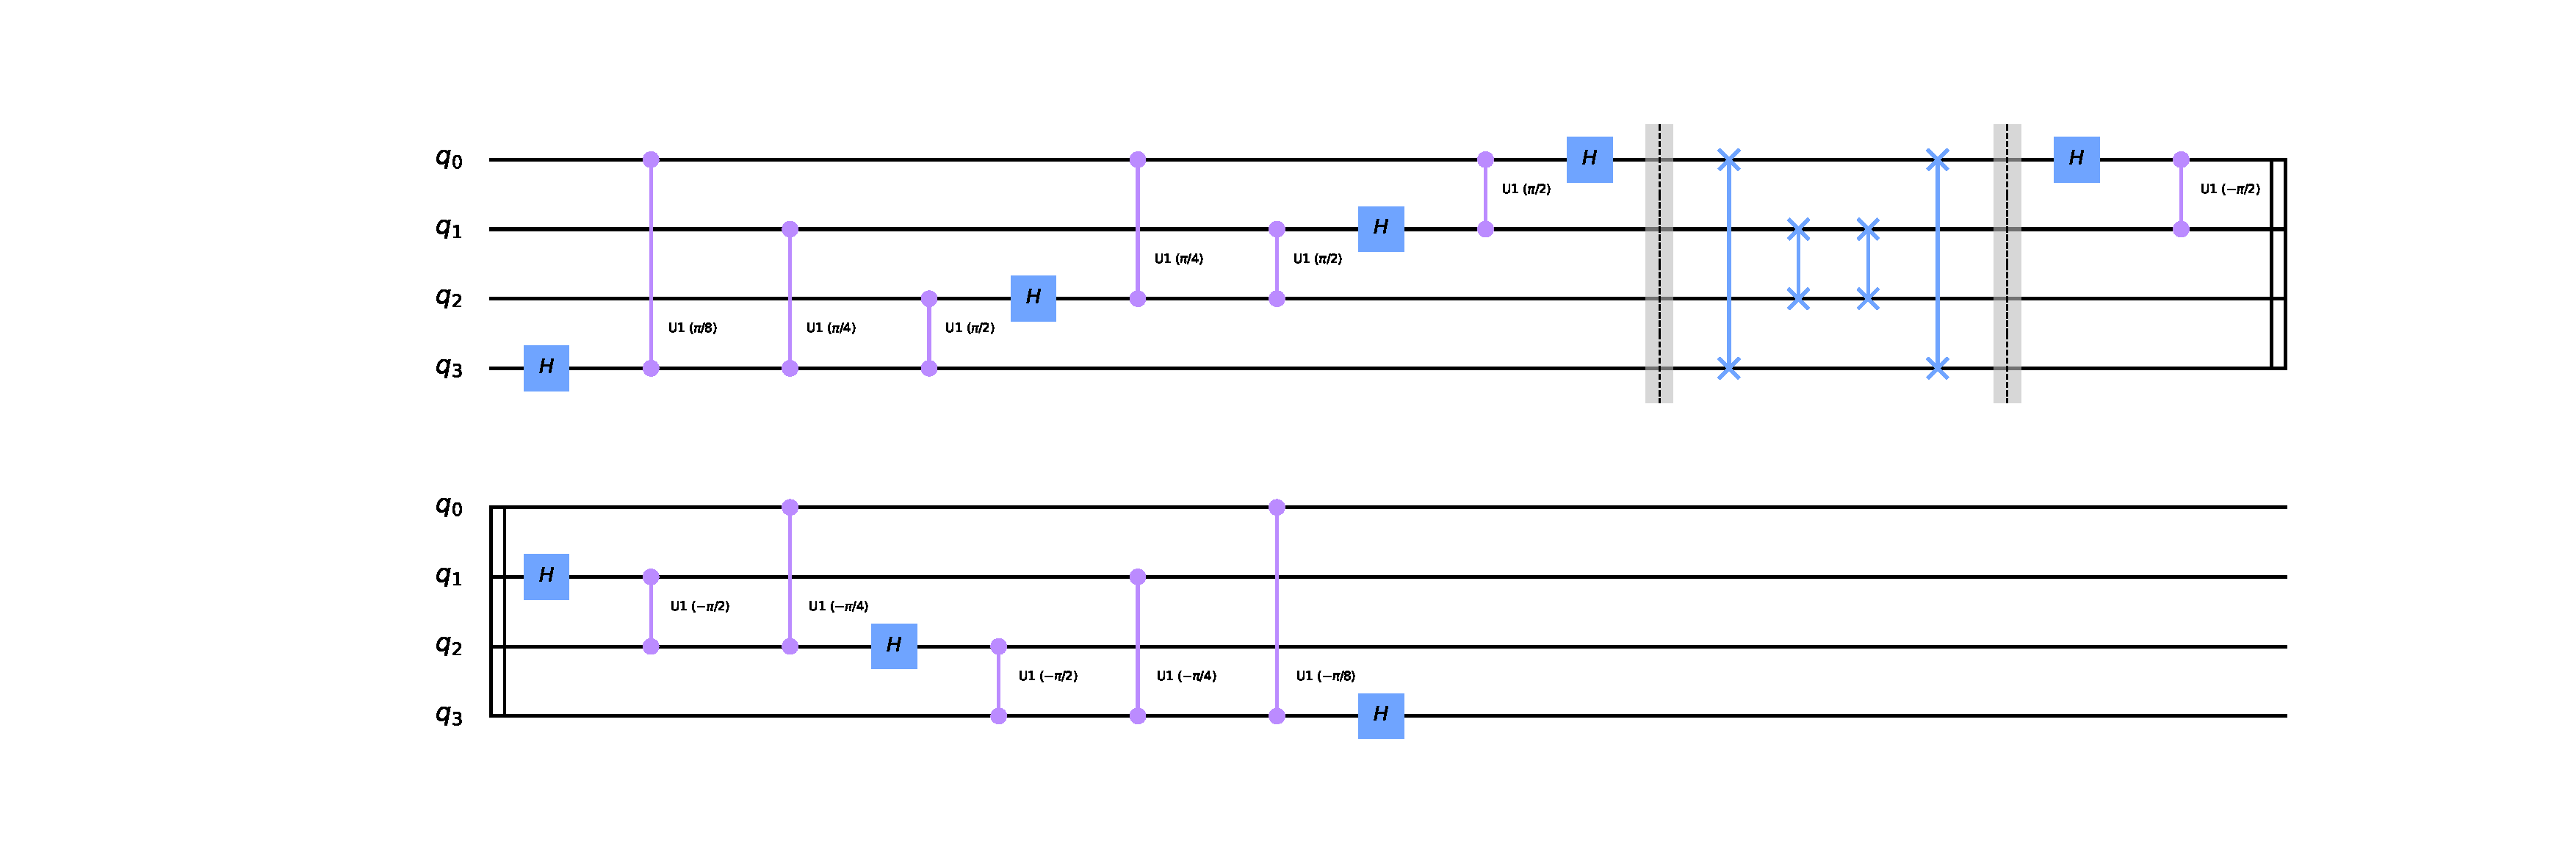
\includegraphics[width=\textwidth]{res/qft-4-qubits-circuit-with-inverse.pdf}
    \caption{Qiskit 4-qubit QFT + inverse QFT circuit}
    \label{fig:qft-4-qubit-circuit-with-inverse}
\end{figure}

The last step to have a fully functional circuit, is to encode a number to the qubits that serve as the input.
A method in appendix~\ref{subsec:encoding-decoding-number-in-circuit} is written that encodes a number to a binary string and later to another quantum circuit that is scaled to fit the amount of needed bits to represent the passed number.
For example the decimal integer number 12 is encoded to the binary string 1100 and therefore needs the circuit to have 4 input qubits.
Additionally, the same code in the appendix shows a function to measure the qubits to classical bits at the end of the circuit to get the circuits result as binary string again.
That result should ideally match the input when no error occurs.

The full circuit for the encoded number \(6\) is shown in figure~\ref{fig:full-qft-3-qubit-circuit}.

\begin{figure}[H]
    \centering
    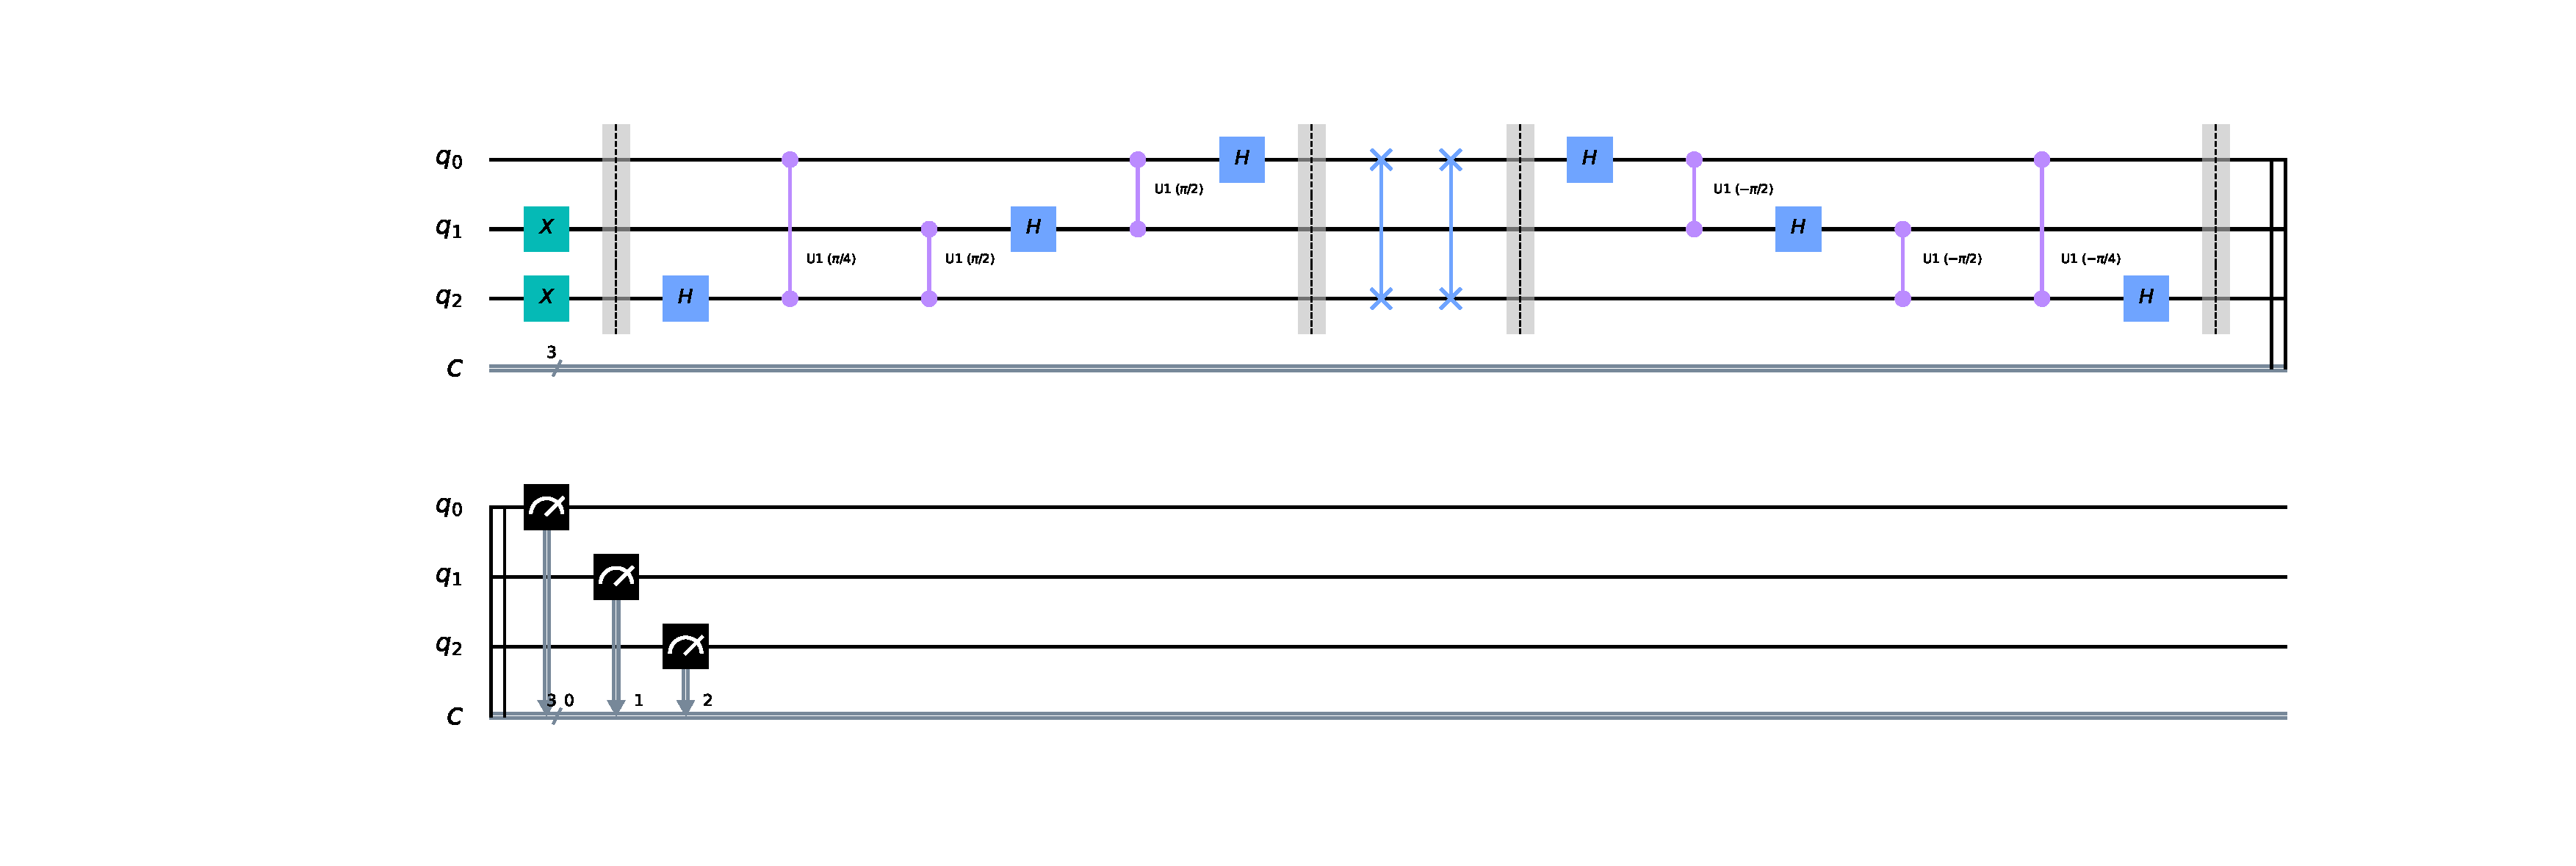
\includegraphics[width=\textwidth]{res/full-qft-3-qubit-circuit.pdf}
    \caption{Qiskit 3-qubit circuit used in this paper}
    \label{fig:full-qft-3-qubit-circuit}
\end{figure}

For the sake of completeness, the source code for generating the above image is listed in Annex~\ref{subsec:generating-full-qft-circuit}.

\paragraph{Testing}

Testing the results of the quantum Fourier transform on a simulator and a real backend.

\subsection{QFT circuit changes for error-correction}
\label{subsec:qft-circuit-error-correction}

\paragraph{Testing}
